\chapter{Introducción criptografía y seguridad informática}
\section{ Definiciones básicas}

 \begin{defn}[Criptografía] Proviene de la palabra griega "oculto". Escribir de forma enigmática.
 \end{defn}
 
 
 \begin{defn}[Texto plano]
 	Texto original.El mensaje que se quiere cifrar está escrito en texto plano
 \end{defn}
 
 
 \begin{defn}[Texto cifrado]
	DIBUJO
 \end{defn}
 
 \begin{defn}[Estenografía]
 	Técnica para esconder mensajes dentro de otro mensaje.
 \end{defn}
 
 
 \section{Contexto histórico de la criptografía}
 
 \subsection{Principales motores de la criptografía}
 
 \begin{itemize}
 	\item Político\item Bélico \item Económico
 \end{itemize}
 
\section{Esquema general de cifrado y servicios proporcionados a la seguridad}

\section{Tipos de ataques}
\section{Modelos y estándares de seguridad informática, auditoría y certificación}

\chapter{Métodos clásicos de cifrado y criptoanálisis}
\section{Definición de criptosistema}
\begin{defn}[Criptosistema]
	Es una quíntupla $(P, C, K, E_k, D_k)$ que satisface
	
\begin{itemize}
	\item $P \rightarrow$ conjunto de textos planos
	\item $C \rightarrow$ conjunto dde textos encriptados
	\item $K \rightarrow$ claves
	\item $E_k(x) \rightarrow$ función de cifrado
	\item $D_k(x) \rightarrow$ función de descifrado
\end{itemize}

\end{defn}
\subsection{Cifrados alfabéticos}
\subsubsection{Cifrado de desplazamiento}

\begin{itemize}
	\item $P\in Z_m$
	\item $C\in Z_m$
	\item $K\in Z_m$
	\item $y=E_k(x)= x+k$ mod m, con $x\in Z_m$ y $K \in Z_m$
	\item $D_k(y) = x- k$ mod m
	
\end{itemize}

La complejidad de descifrado depende de $|K|$, en este caso
$$|K| = |Z_m| = m$$
Vemos que $E_k$ y $D_k$ son muy rápidas, por lo que se pueden ejecutar en tiempo real, pero a la vez es muy fácil de descifrar.

\subsubsection{Cifrado de sustitución}

\begin{itemize}
		\item $P\in Z_m$
		\item $C\in Z_m$
		\item $K \rightarrow$ permutación de símbolos
		\item $y=E_k(x)= \Pi(x)$ ($\Pi \rightarrow$ permutación)
		\item $D_k(y) = \Pi^{-1}(y)$
\end{itemize}

Es importante ver que en $Pi$ no puede haber índices repetidos.
\begin{example}
	
	
	\textbf{\\ \\ Bien:}
	
	$\begin{matrix}
		1 & 2 & 3 & 4\\
		2 & 1 & 3 & 4
	\end{matrix}$
	
	\textbf{\\ Mal:}
	
		$\begin{matrix}
		1 & 2 & 3 & 4\\
		1 & 1 & 3 & 4
		\end{matrix}$
	
	
\end{example}

Este cifrado es más complejo ya que $|K| = m!$

\subsubsection{Cifrado afín}

\begin{itemize}
	\item $P\in Z_m$
	\item $C\in Z_m$
	\item $K \in (a,b)$
	\item $y=E_k(x)= ax + b$ mod $m , a\in Z^*_m$ y $b\in Z_m$
	\item $D_k(y) = (y-b)* a^{-1}$ mod $m$
\end{itemize}

Decimos que $ a\in Z^*_m$ ya que si $ a\in Z_m$, entonces $a^{-1}$ no tiene porqué existir. Por esto definimos
$$Z^*_m = \{a\in Z_m | mcd(m,a) = 1\}$$

Esto nos asegura que $\forall a \in Z^*_m $ existe $a^{-1}$

Para saber que $a$ queremos utilizar, tenemos que ver:
\begin{enumerate}
	\item mod(a,m) = 1. Para comprobar esto utilizamos el algoritmo de Euclides.
	
	\item ¿Cómo hallamos $a^{-1}$? . Para esto utilizaremos el algoritmo de Euclides extendido.
\end{enumerate}

\begin{enumerate}
	\item \textbf{mcd(a,m) = mcd(m, a mod m)}\\
	
	
	\underline{EUCLIDES}
	
	Llamamos $r_0 = a$ y $r_1 = m$
	
	$r_0 = q_1 r_1 + r_2$, de forma que $mcd(r_0,r_1) = r_2$
	
	$r_1 = q_2 r_2 + r_3$
	
	$\dots$
	
	$r_{n-2} = q_{n-1}r_{n-1} + r_n$
	
	$r_{n-1} = q_{n}r_{n}$
	
	Y asi nos queda que
	$$r_n = mcd (a,m)$$
	
	\item \textbf{¿ $a^{-1}$?}\\
	
	\underline{EUCLIDES EXTENDIDO}
	
	La idea es escribir el algoritmo de Euclides pero escribiendo todos los restos en función de $a$ y $m$.
	
	Llamamos $r_0 = a$ y $r_1 = m$
	\begin{itemize}
		\item $r_0 = q_1 r_1 + r_2 \implies r_2 = r_0 - q_1 r_1 \implies r_2 = a-q_1m$
		
		\item $r_1 = q_2 r_2 + r_3 \implies r_3 = m - q_2 r_2$ , y como $r_2$ está e función de $a$ y de $m$ , entonces $r_3 = m(1+q_1q_2) - q_2a$
		
		\item $r_4 = r_2 - q_3 r_3$
		
		$\dots$
		
		\item $r_{n} = m\cdot U_n + a\cdot V_n \implies a \cdot V_n = 1$ mod $m \implies a^{-1} = V_n$
		
	\end{itemize}
	
	Ejercicio: ¿Cómo calculamos esa $V_n$?
	
	 $r_0 = r_0$\\ $r_1 = r_1$\\$r_2 = r_0 -q_1r_1$\\$r_3 = -q_2r_0 + (1+q_1q_2)r_1$\\ $r_4 = (1+ q_3q_2)r_0 -(q_1 +q_3(1+q_2q_1))r_1$\\ ... \\ Llamamos al término que acompaña al $r_0$ : $U_i$ y al término que acompaña al $r_1$ : $V_i$\\ 
	 
	 Para calcular $U_i$ cogemos $U_0=1$ , $U_1 = 0$ y calculamos:
	 $$U_i = U_{i-2} - q_{i-1}U_{i-1} \iff i\geq 2$$
	
	 Para calcular $V_i$ cogemos $V_0=0$ , $V_1 = 1$ y calculamos:
	 $$V_i = V_{i-2} - q_{i-1}U_{i-1} \iff i\geq 2$$
	 
	 \begin{example}
	 Euclides (a,b)	 
	 	
	 	$r_0 \leftarrow a$\\$r_1\leftarrow b$\\$m\leftarrow 1$
	 	
	 	while $r_m \neq 0$
	 	
	 	 do 
	 	$\begin{cases}
	 		q_m \leftarrow \lfloor\frac{r_{m-1}}{r_m}\rfloor\\ r_{m+1} \leftarrow r_{m-1} - q_mr_m\\m\leftarrow m +1
	 		
	 	\end{cases}$
	 	
	 	$m\leftarrow m-1$
	 	
	 	return ($q_1,...,q_m; r_m$)
	 \end{example}
	 
\end{enumerate}
 \begin{theorem}[Teorema Fundamental de la Aritmética]
 	Todo número se puede descomponer en un producto de números primos.
 	$$m = \Pi^{n}_{i-1} \cdot p^{e_i}_{i}$$
 	
 \end{theorem} 
 
 \begin{theorem}[Función de Euler]
 	La función de Euler nos indica el número de coprimos a uno dado.
 	$$\phi(m) = |Z^{*}_m| = \Pi{n}_{i=1} (p^{e_i}_i - p^{e_i-1}_i)$$
 	
 \end{theorem}
 

 
 \begin{example}
 	Vamos a buscar cuantas claves tenemos en español (27 letras)
 	$$K = |Z_{27}| x |Z^{*}_{27}| = 27\cdot 18 = 486$$
 \end{example}


Vamos a ver una forma de calcular el inverso multiplicativo con Euler generalizado, esta forma no vale para números grandes.

\begin{theorem}[Euler generalizado]
	$$\text{a} \in Z^{*}_m \implies a^{\phi(m)} \equiv 1 \text{ mod } m$$
\end{theorem}

\textbf{Truco para inverso}:

$$a^{\phi(m)} = a^{\phi(m) - 1} \cdot a \equiv 1 \text{ mod } m$$
$$...$$
$$a^{\phi(m) -1} = a^{-1} \text{ mod } m$$

\textbf{¿Porqué no se utiliza esta forma de calcular en inverso?} Porque necesitamos $\phi(m)$ , que se calcula con la descomposición en números primos, y esto no es trivial para números grandes.

Hasta ahora hemos estado viendo cifrados alfabéticos, es decir, que vamos cifrando cada letra del mensaje plano con una clave, de forma que nos queda el mensaje cifrado.


A partir de ahora vamos a ver cifrados en bloque

\subsection{Cifrados en bloque}

\subsubsection{Cifrado de Vigenere}

\begin{itemize}
	\item $P= Z_m \times Z_m \times ..... \times Z_m = (Z_m)^{n}$
	\item $C = (Z_m)^{n}$
	\item $K = (Z_m)^{n} = P = C$
	\item $E_{\overrightarrow{k}} = E_{k_1,...,k_n}(\overrightarrow{x}) = (x_1+ k_1,...,x_n+ k_n) \text{ mod } m \equiv Y$
	\item $D_{k_1,...,k_n} ( \overrightarrow{Y}) = (y_1- k_1,...,y_n- k_n) \text{ mod } m $
\end{itemize}

\subsubsection{Cifrado de Hill}

\begin{itemize}
	\item $P= (Z_m)^{n}$
	\item $C = (Z_m)^{n}$
	\item $K$ es una matriz $n \times n$
	\item $\overrightarrow{y} = E_{k}(\overrightarrow{x}) = (x_1,....,x_n) \cdot K \text{ mod } m$
	\item $D_{k}(\overrightarrow{y})= (y_1,....,y_n) \cdot K^{-1}_{n \times n}$
\end{itemize}
\paragraph{Condiciones para este criptosistema}
\begin{enumerate}
	\item det($K$)$\neq 0$ $\implies$ esto es para que exista $K^{-1}$
	\item mcd (det($K$) , $m$)$= 1$
\end{enumerate}

\subsubsection{Cifrado de permutación}
\begin{itemize}
	\item $P= (Z_m)^{n}$
	\item $C = P$
	\item $K$ es un vector de permutación $\overrightarrow{\Pi}$ de n permutaciones
	\item $E_{k}(\overrightarrow{x}) = (x_{\Pi(1)},....,x_{\Pi(n)})= Y$
	\item $D_{k}(\overrightarrow{y})= (y_{\Pi(1)},....,y_{\Pi(n)}$
\end{itemize}

\begin{example}
	
	$n=6$
	
	$$\begin{matrix}
	x = & 1 & 2 & 3 & 4 & 5 & 6\\
	\Pi(x) = & 3 & 5 & 1 & 6 & 4 & 2\\
	\end{matrix}$$
	
	$$\begin{matrix}
	y = & 1 & 2 & 3 & 4 & 5 & 6\\
	\Pi(y)^{-1} = & 3 & 6 & 1 & 5 & 2 & 4\\
	\end{matrix}$$
\end{example}

Es muy sencillo transformar un \textit{Cifrado de Permutación} en un \textit{Cifrado de Hill}. Vamos a ver como:

\begin{example}
	
	Estamos en $Z^3_n$ , la permutación es $\Pi = (3,2,1)$.
	
	$\begin{matrix}
		x\rightarrow & 1 & 2 & 3\\
		\Pi(x)\rightarrow & 3 & 2 & 1\\
	\end{matrix} \iff \begin{matrix}
	(x_1 & x_2 & x_3)
	\end{matrix} \left(\begin{matrix}
		0 & 0 & 1\\ 0 & 1 & 0\\ 1 & 0 & 0
	\end{matrix}\right) = \begin{matrix}
	(x_3 & x_2 & x_1)
	\end{matrix}$
\end{example}

\subsection{Cifrados de flujo}

Hay dos tipos de cifrados de flujo:
\begin{itemize}
	\item \textbf{Síncronos} $\rightarrow$ K independiente de M
	\item \textbf{Asíncronos} $\rightarrow$ si K depende de las claves anteriores
\end{itemize}

En este tipo de cifrado la transformación va a ser del tipo:

$\begin{matrix}
 X \sim & X_1 & X_2 & ....\\
 Z \sim & Z_1 & Z_2 & ....\\
\end{matrix} \implies \begin{matrix}
y \sim & e_{Z_1}(x_1) & e_{Z_2}(x_2) & ....\\
\end{matrix}$

\begin{example}[Cifrado síncrono de flujo periódico de periodo d]
	\begin{itemize}
		\item $P= C = Z_n$
		\item $e_Z(x) = x + Z$ mod $m$
		\item $d_Z(x) = x - Z$ mod $m$
		\item $Z \rightarrow$ es el flujo de claves $\implies Z = Z_1Z_2...$
		
		$Z_i \begin{cases}
			K_i \text{ si } 1 \leq i \leq 1\\
			Z_{i-n} \text{ si } i \geq n+1
		\end{cases}$ 
		
		Al ser cifrado de flujo periódico de periodo d $\implies Z_{i+d} = Z_i$ 
	\end{itemize}
	\begin{remark}
		El los \textbf{Alfabetos binarios},  $e_Z(x) = x + Z$ mod $2$ , que es lo mismo que hacer un XOR
	\end{remark}
\end{example}




\subsubsection{Generador de claves}

 Para obtener seguridad en los dispositivos hardware , se emplean registros de desplazamiento retoralimentados como generadores de números pseudoaleatorios para las claves de cifrados de flujo.
 
 Estos registros pueden ser:
 
\begin{itemize}
	\item LFSR $\rightarrow$ registros de desplazamiento con retroalimentación lineal
	\item NLFSR $\rightarrow$ registros de desplazamiento con retroalimentación no lineal
\end{itemize}

Con esto generamos una \textbf{key stream}.

\textbf{¿Cómo funciona?}
\begin{enumerate}
	\item Primero generamos una clave : $Z_i = K_i$  $1< i \leq n$ ; $c = (c_0, c_1....c_{n-1}) \implies K = (K_1, K_2,..., K_n,c_0....c_{n-1})$
	\item Recurrencia (de orden n). Un ejemplo es
	$$Z_{i+n} = \sum_{j=0}^{n-1} c_j \times Z_{i+j} \text{ mod } 2$$
\end{enumerate}

\begin{example}[RC4]
	\begin{center}
		\Tree[.ClaveSecreta [.RC4 [.KeyStream [.Tp$\to\oplus\to$Tc ] ] ] ]
	\end{center}
\end{example}

\begin{problem}
	Hallar el orden de recurrencia de la siguiente clave:
	$$(1000,1100)$$
	
	\solution Se deja como ejercicio para el lector. El orden deberá salir 15.
	
\end{problem}

\subsection{Producto de Criptosistemas}
Se define de la siguiente forma:


	$S_1 = [ P, C, K_1 E_{K_1} D_{K_1}]$
	
	$S_2 = [ P, C, K_2 E_{K_2} D_{K_2}]$
	
	$$S_1 \times S_2 = [ P, C, K_1 E_{K_1} D_{K_1}] \times [ P, C, K_2 E_{K_2} D_{K_2}] = [ P, C, K_1 \times K_2, E_{K_1 K_2} D_{K_1 K_2}]$$
	
	\begin{problem}
		Combina los siguientes criptosistemas:
		$$\begin{cases}
		 y = x + K_1 \text{ mod } m\\
		 y = x + K_2 \text{ mod } m\\
		\end{cases}$$
		\solution
		$E_{K_2}(E_{K_1}(x)) = E_{K_2}(x + K_1) = x + K_1 + K_2$
	\end{problem}
	
	\begin{problem}
		Combina los siguientes criptosistemas y halla la robusted del criptosistema resultante
		$$\begin{cases}
		y = x + b\\
		y= ax\\
		\end{cases}$$
		
		\solution
		\begin{itemize}
			\item $E_{K_2}(E_{K_1}(x)) = E_{K_2}(x + b) = a \cdot(x + b) = ax + ab$
			
			Como $ab \in Z_m$ llamamos $ab = \beta \in Z_m$ de forma que el producto de los criptosistemas nos queda:
			$$ax + \beta \text{ mod } m$$
			\item Para calcular la robusted vemos que 
			\begin{itemize}
				\item $|b| = m$
				\item $|a| = |Z^{*}_m| = \phi(m) \text{ mod } m$
			\end{itemize}
			Ahora ya podemos calcular la robusted del producto
			$$|a| \cdot |\beta| = |Z^{*}_m| \cdot |Z_m| = \phi(m) \cdot m$$
		\end{itemize}
			
	\end{problem}
	
\begin{remark}
Combinar cifrados de sustitución con permutación ha dado lugar a cifrados como : \textbf{CRIPITO, DES, AES...} 
\end{remark}

\section{Tipos de ataques}

\subsection{Criptoanálisis}
En el criptoanálisis el algoritmo es conocido.

Del criptoanálisis deriban las \textbf{Reglas de Kerchhoffs}
\begin{enumerate}
	\item Algoritmo de cifrado público
	\item La fortaleza del criptograma reside en K(clave)
\end{enumerate}

Vamos a ver los supuestos ataques con los que podeos encontrarnos

\begin{itemize}
	\item[A)] Solo texto cifrado $\rightarrow$ es el caso más difícil.
	\item[B)] Texto claro conocido $\rightarrow$ texto cifrado + pareja plano-cifrado 
	\item[C)] Texto claro elegido $\rightarrow$ texto cifrado + pareja plano elegida-cifrado
	\item[D)] Texto cifrado elegido $\rightarrow$ texto cifrado + pareja plano-cifrado elegido 
	\item[E)] Texto elegido 
\end{itemize}

\subsubsection{Cifrado de desplazamiento}

Este cifrado se rompe de forma \textbf{inmediata} en los supuestos \textbf{B, C, D} y \textbf{E}.

En el caso \textbf{A} no es inmediato pero también es sencillo. Se hace utilizando las estadísticas del idioma.

\begin{example}[Supuesto A-] 
	
	Sabemos que la letra que más se usa en el español es la E ($16'.. \%$) , si en nuestro texto cifrado la letra más repetida es la D, es lógico pensar que $e_K(E) = D$.
	
	A partir de aquí es fácil hallar la clave.
	
	Si vemos que el resultado es un texto sin sentido, cambiaremos nuestra hipótesis(en función de las estadísticas) y seguiremos probando.
\end{example}


\subsubsection{Cifrado Afín}

Este cifrado se rompe de forma \textbf{muy sencilla} en los supuestos \textbf{B, C, D} y \textbf{E} si tengo dos parejas de texto plano-cifrado (x-y)
$$\begin{cases}
x_1 - y_1\\
x_2 - y_2
\end{cases} \rightarrow \begin{cases}
y_1 = x_1 + b \text{ mod }m\\
y_2 = x_2 + b \text{ mod }m\\
\end{cases}$$
Y resuelvo el sistema.

En el caso \textbf{A} no es tan sencillo pero con estadística también se puede romper. Si la primera hipótesis falla, probaremos con la siguiente letra más probable hasta dar con un texto que tenga sentido.

\subsubsection{Cifrado de Sustitución}

Este es más complicado, necesitaremos estadísticas más completas (COMPLETAR DEL LIBRO)

\subsubsection{Cifrado de Vigenere}

$$\overrightarrow{y} = \overrightarrow{x} + \overrightarrow{K} \text{ mod } m$$

Para analizar esto una simple estadística no vale, porque dependiendo de cual sea  la longitud de la clave, \textbf{mismos textos se cifran de forma diferente}.

Por lo tanto el criptoanálisis se hace en dos pasos:
\begin{enumerate}
	\item\textbf{ Hallar el tamaño de la clave $\rightarrow$ ¿n?}
	
	Para esto podemos utilizar dos métodos $\begin{cases}
	KASISKI \rightarrow 1863\\
	\textit{Índice de coincidencia}\\
	\end{cases}$
	\begin{itemize}
		\item \textbf{KASISKI} $\rightarrow$ Se basa en la suposición de que puede haber repeticiones en el texto cifrado que vengan de la misma parte del texto plano.
		
		\begin{enumerate}
			\item localizamos las repeticiones y las llamamos $Y_1$
			\item llamamos a la posición de inicio de cada repetición $i_1, i_2,i_3...$
			\item llamamos la distancia entre las repeticiones $\delta_1 , \delta_2....$
			\item vemos que :
			
			$\begin{cases}
			i_2 = i_1 + K_1\cdot n\\
			i_3 = i_2 + K_2\cdot n\\
			....\\
			\end{cases}$ 
			
			COMPLETAR!!!!
		\end{enumerate}
		\item \textbf{Índice de coincidencia} $\rightarrow$ Dado una cadena de datos $\overrightarrow{X} = X_1 X_2 .... X_l$, el índice de coincidencia de dicha cadena $I_c(\overrightarrow{X})$ es la probabilidad de que dos elementos de esa cadena coincidan.
		
		Supongamos que tenemos una serie de caracteres en $\overrightarrow{X}$ con frecuencias de ocurrencia $f_0,f_1, f_2 ....$.
		
		Nos preguntamos: ¿De cuantas formas podemos combinar un caracter $X_i$ en dicha cadena?
		$$\comb{f_i}{n}$$
		¿De cuantas formas podemos coger n $X_i$ iguales?
		$$\sum_{i} \comb{f_i}{n}$$
		
		\begin{remark}
			Supongamos que tenemos n objetos y queremos elegir los objetos de $r$ en $r$ sin atender a la ordenación de los mismos.
			
			El número de combinaciones que existen de n objetos tomados de $r$ en $r$ es $\comb{r}{n}$
		\end{remark}
		

		
		Por lo tanto el caso de mayor $I_c(X)$ es el caso en que la cadena tenga todos los caracteres iguales.
		
		Una vez visto todo esto podemos definir el $I_c(X)$ como:
		$$I_c(\overrightarrow{X}) = \frac{\sum_{i}\comb{f_i}{2}}{\comb{l}{2}} = ... = \frac{\sum_{i} f_i \cdot (f_i -1)}{l\cdot(l-1)} = \sum_{i} \frac{f_i}{l} \cdot \frac{f_i-1}{l-1} $$
		
		Si nos fijamos:
		
		$\frac{f_i}{l} = P_i$ es la probabilidad de cada letra y $\frac{f_i-1}{l-1} \sim P_i$, por lo tanto
		$$I_c(\overrightarrow{X}) \sim \sum_{i} P^2_i$$
		
		Este índice lo hemos calculado para los 1-gramas.
		
		\begin{defn}[n-grama]
 composición de n símbolos de un lenguaje
		\end{defn}
		
		\begin{example}
			Vamos a ver el índice de coincidencia de un lenguaje aleatorio y el del inglés:
			$$I_c(\overrightarrow{X})_{aleatorio} = 0.038$$
			$$I_c(\overrightarrow{X})_{inglés} = 0.065$$
		\end{example}
		
		
	\textbf{Y con esto, ¿cómo calculamos el número de claves?}
	
	\begin{example}
		
		Tamaño de $\overrightarrow{K} = n$ ,	$\overrightarrow{K} = \{K_1, K_2, ....\}$
		Sabemos que estamos en el cifrado de Vigenere.
		
		\textbf{Pregunta: ¿n?}
		
		Vamos a hallarla con el $I_c(\overrightarrow{x})$
		
		$$M_c = y_1...y_n' , y_{n'+1}.....y_{2n'} , y_{2n'+1}....y_{3n'},....y_l$$
		
		$$\begin{cases}
			\overrightarrow{X_1}= y_1, y_{n'+1}, y_{n'+2}...\\
			\overrightarrow{X_2}= y_2, y_{n'+2}, y_{2n'+2}...\\
			.....\\
			\overrightarrow{X_n}= y_{n'}, y_{2n'}, y_{3n'}...\\
		\end{cases}$$
		
		¿Cómo sabemos si $n' = n$? Podemos ir probando con diferentes $n'$, el correcto será el que de un $I_c$ similar al del lenguaje en el que esté el mensaje en claro.
	\end{example}
	
	\end{itemize}
	\item \textbf{Descubrir las $K_i$}
	
	Para esto también podemos utilizar el $I_c$.
	
	\textit{\textbf{La idea es:} Si mi clave es de longitud 3, cojo el mensaje cifrado y cojo los caracteres 1,4,7,10...(esto es $X_1$) y sabemos que todos esos caracteres han sido cifrados con la misma letra. Ahora vamos probando distintas letras (claves), sobre dichos caracteres y calculamos su $I_c$, de nuevo cuando el $I_c$ coincida con el del idioma en el que está escrito el mensaje, tendremos la clave correcta. Hacemos esto con cada $X_i$}
	
	Lo primero que hacemos es calcular todas las frecuencias de esa cadena, $f_j : 0 \leq j < m$
	
	Vemos que la longitud de cada $\overrightarrow{X}_i$ es $\frac{l}{n}$ y el número de símbolos del lenguaje es $m$
	
	$$I_c(\overrightarrow{X}) = \sum_{j=0}^{m-1} p_j \cdot \frac{f_{j-K_i}}{\frac{l}{n}} = M(K_i)$$
	
	$$M_g = \sum_{j=0}^{m} p_j \frac{f_{j+g}}{l/n} = M(K_i)$$ 
	\begin{example}
		
		Contrastar que $\sum_{i}^{m-1} p_i p_{i-l} = \sum_{i}^{m-1} p_i p_{i+l}$
		
	\end{example}
	
	\begin{problem}[5]
		Probar que $y = a\cdot b$ mod $m$ constituye un criptosistema siempre y cuando $mcd(a,m) = 1$
		
		\solution
		Vamos a suponer 2 casos:
		
		\underline{CASO 1} : $mcd(a,m) = 1$
		$$\begin{cases}
		y_1 = ax_1 + b\\y_2= ax_2 +b
		\end{cases} \implies a(x_1 - x_2) = 0 \text{ mod } m $$
		
		Entonces
		
		$$a(x_1 - x_2) = q \cdot m \implies q = \frac{a(x_1 -x_2)}{m}$$
		
		tal que m \textbf{no divide} a $a$ $\implies m>a$
		
		También vemos que m \textbf{no divide} a $x_1 - x_2$ ya que ambos pertenecen a $Z_m$ por lo tanto ambos serán más pequeños que $m$.
		
		
		
		\underline{CASO 2} : $mcd(a,m) = d > 1$ de forma que $d$ divide a $a$ y $m$.
		
		$a(x_1 - x_2) = 0 \text{ mod } m$
		
		Llamamos $a_d = \frac{a}{d}$ y $m_d = \frac{m}{d}$
		
			$$a(x_1 - x_2) = q \cdot m \implies a_d(x_1 - x_2) = q \cdot m_d$$
			
			$$q = \frac{a_d(x_1 -x_2)}{m_d}$$
			
			Vemos que $m_d$ no divide a $a_d$ porque $m_d > a_d$
			
			¿Puede dividir $m_d$ a $(x_1-x_2)$ ?  Si, porque $m_d <m$
		
	\end{problem}
	
\end{enumerate}
 \subsubsection{Cifrado de Hill}
 
 \begin{problem} Ejercicio 9 del libro
 	
 	Vamos a calcular el número de claves en el criptosistema de Hill.
 	
 	Supongamos que la matriz
 	$$M_K = ( \begin{matrix}
 	K_{11} & K_{12}\\
 	K_{21} & K_{22}
 	\end{matrix} ) $$
 	
 	Determinante de $M_K \neq 0$ , mcd(det($M_K$),$P$)$= 1$ , siendo $P$ primo.
 	\solution
 	
 	Vemos que cuando $P$ es primo y det$\neq 0$, siempre se cumple que son coprimos.
 	
 	
 	
 \end{problem}
 
 % % Parte de Jose
 
 \chapter{Cifrado perfecto y distancia de unicidad}
 
 \textbf{1949}$\rightarrow$ Sientan las bases teóricas del cifrado automático (Claude Shannon).
 
 \section{Seguridad perfecta}
 
 En este capítulo veremos dos temas, siempre basándonos en que nos encontramos en el \textbf{caso A} (solo tenemos el texto cifrado).
 
 \begin{itemize}
 	\item \textbf{SEGURIDAD PERFECTA}
 	\begin{itemize}
 		\item \textbf{Seguridad Computacional}
 		\begin{itemize}
 			\item Análisis que se hace a los algoritmos criptográficos para ver cómo romperlos.
 			\item  Intenta aproximar cuantas operaciones necesitas hacer para poder romper el sistema(averiguar la clave).
 			\item Un buen criptosistema es quel cuyo tiempo de uso es mucho menos que el tiempo que necesitamos para romperlo.
 			
 		\end{itemize} 

 		\item \textbf{Seguridad incondicional}
 		\begin{itemize}
 			\item Modelo en el que tenemos una máquina con recursos ilimitados, esta no es capaz de romper el criptosistema.
 		\end{itemize}
 	\end{itemize}
 	
 \end{itemize}


\begin{remark}
	Antes de seguir con segurdad perfecta vamos a repasar algunos conceptos de probabilidad que nos serán utiles en el estudio de este tema.
	
	Tenemos $x \in X = \{ x_1,....x_n\} , y \in Y = \{ y_1,...y_n\}$
	
	Llamamos $P(x = x_1) = P_p(x)$ y $P(y = y_1) = P_c(y)$
	
	Probabilidad conjunta:
	
	$$P(x,y) = P(x|y)\cdot P(y)$$
	
	y calculamos $P(x|y)$ de la siguiente forma:
	$$P(x|y) = \frac{P(x,y)}{P(y)} = \frac{P(y|x) \cdot P(x)}{P(y)} = \frac{P(y|x) \cdot P(x)}{\sum_{x} P (y|x)P(x)}$$
	
	
	Ahora vamos a aplica esto a los criptosistemas:
	
	$$P_p(x) ; x \in P \rightarrow\text{  P = texto plano}$$
	$$P_k(k) ; k \in K \rightarrow\text{  K es el conjunto de claves}$$
	
	Si tenemos independencia entre x y k $ \implies P(x,k) = P_p(x)P_k(k)$
	
	¿Y como calculamos $P_c(y)$?
	
	$$P_c(y) \underbrace{=}_{\text{bayes}} \sum_{k}P(x,k,y) = \sum_{xk} P(y|xk) \cdot P(xk) \underbrace{=}_{\text{IE}} \sum_{xk} P(y|xk)P_p(x) P_k(k)$$
	
	$$P(y|xk) = \begin{cases}
		\text{Si } e_k(x) = y \implies P(y|xk) = 1\\
		\text{Si } e_k(x) \neq y \implies P(y|xk) = 0\\
	\end{cases} \implies \textbf{Esto es la condición de criptosistema}$$
	
	Por lo tanto:
	$$\sum_{\forall x,y,k| y = e_k(x)} P_p(x) \cdot P_k(k) = P_c(y)$$
	
	Vamos a ver como se calcula la \textbf{probabilidad a priori}
	$$P_c(y|x) = \frac{P(y,x)}{P_p(x)} = \frac{\sum_{k}P(y,x,k)}{P_p(x)} = \frac{\sum_{k}P(y|kx)\cdot P(xy)}{P_p(x)} =$$
	 $$ =\frac{\sum_{k}P(y|kx)\cdot P_p(x)P_k(k)}{P_p(x)} = \sum_{k}P(y|kx)\cdot P_k(k)$$
	$$ \sum_{\forall k | e_k(x)=y} P_k(k) = P_c(y|x)$$
	
	Y ahora la \textbf{probabilidad a posteriori}
	$$P_c(x|y) = \frac{P_p(x) P_c(y|x)}{P_c(y)} = \frac{P_p(x) \sum_{\forall k| e_k(x) = y}P_k(k)}{\sum_{\forall x,k| e_k(x) =y} P_p(x) P_k(k)}$$
	
\end{remark}

\begin{defn}[Seguridad Perfecta]
	Decimos que un criptosistema tiene seguridad perfecta si cumple:
	$$P_p(x|y) = P_p(x)$$
	Esto quiere decir que el conocimiento de texto cifrado no nos da ninguna información sobre el texto plano.
\end{defn}

 Si tuvieramos el texto plano seria muy facil romperlo, pero tenemos que recordar que seguimos estando el el supuesto A (solo texto cifrado).

\begin{example}
	Supongamos que tenemos un texto plano $P=\{a,b\}$ tal que $P(a = 1/4)$ , $P(b) = 3/4$.
	
	Tenemos $K=\{k_1,k_2,k_3\}$ tal que $P(k_1) = 1/2$ , $P(k_2) = P(k_3) = 1/4$ y $c = \{1,2,3,4\}$

	
\begin{center}
		
	\begin{tabular}{l | c  r}
		  & a & b\\
		\hline
		$k_1$ & 1 & 2 \\
		$k_2$ & 2 & 3 \\
		$k_3$ & 3 & 4 \\
	\end{tabular}
\end{center}
	
		¿Cumple la seguridad perfecta?
		
		Vamos a calcular la probabilidad de que me salga cada uno de los elementos del texto cifrado:
	
	$$P_c(1) = P_p(a) P_k(k_1) = 1/8$$
	$$P_c(2) = P_p(a) P_k(k_2) + P_p(b) P_k(k_1) = 7/16$$
	$$P_c(3)= 1/4$$
	$$P_c(4) = 3/16$$
	Ahora vamos a mirar la probabilidad a priori de ese texto cifrado:
	
	$$P_c(1|a) = P_k(k_1) = 1/2$$
	$$P_c(2|a) = P_k(k_2) = 1/4$$
	$$P_c(3|a) = P_k(k_3) = 1/4$$
	$$P_c(4|a) = P_k(k_4) = 0$$
	
	$$P_c(1|b) = 0$$
	$$....$$
	
	y asi todo el rato
	
	Vamos a por la posteriori:
	$$P_p(a|1) = \frac{P_c(1|a) \cdot P_p(a)}{P_c(1)} = 1$$
	$$P_p(a|2) = \frac{1/16}{7/16}$$
	
	y asi todo el rato...
	
	Podeos ver que no es un criptosistema con seguridad perfecta.
\end{example}


\begin{example}
 	

Supongamos m claves del cifrado de desplazamiento que se que se ... con $P_k(k) = 1/m$ para cualquier $P_c(k)$

$$|P| , |C| , |K| = m$$

	\begin{center}
		
	\begin{tabular}{l | c | r}
		k|x & 0 & 1\\
		\hline
		0 & 0 & 1 \\
		\hline
		1 & 1 & 0\\
	
	\end{tabular}
\end{center}
	
	$$P_c(y) = \sum_{x,k | e_k(x) = y} P_p(x) P_k(x) = \frac{1}{m} \sum_{x|e_k(x) = y} P_p(x) = \frac{1}{m} \sum_{x=0}^{m-1} P_p(x) = \frac{1}{m} = P_c(y)$$


	$$P_c(y|x) = \sum_{k|e_k(x) = y; y= x+k} P_k(k) = \frac{1}{m}$$
	
	Y ya lo tenemos porque ahora podemos hacer la condicionada.
	
	$$P(x|y) = \frac{P(y|x) P (x)}{P(y)} = \frac{P(x) 1/m}{1/m} = P(x)$$
 \end{example}
 
 El criptosistema utilizado en el ultimo ejemplo es el \textbf{cifrado de vernan u OTP(one-time pad)}
 
 
 
 \underline{\textbf{Cifrado de OTP}}
 \begin{center}

 $M_p = x_1,....,x_n$\\
 $K= k_1,...,k_n \rightarrow P(k_1) = \frac{1}{k}$\\
 $M_c = y_1,...,y_n ; y_i = x_i + k_i$\\
 $|P| = |C| = |K| = m$
  	
  \end{center}
 
 Cuando se utilizaba este cifrado mandaban el mensaje por un canal inseguro y la clave por un canal seguro
 
 $$E \rightarrow P \rightarrow x+k = y \rightarrow \text{Canal Inseguro} \rightarrow Receptor$$
 $$\text{Generador de Claves} \rightarrow k \rightarrow \text{Canal Seguro} \rightarrow Receptor \rightarrow y-k \rightarrow P$$
 
 \begin{theorem}[Teorema cifrado perfecto]
 	Dado $[P,C,K,E_K,D_K]$ donde $|P| = |C| = |K|$ este proporciona seguridad perfecta si y solo si:
 	\begin{enumerate}
 		\item $P_k (k) = \frac{1}{|k|} ,  k\in K$
 		\item $\forall x \in P , \forall y \in C$ hay una sola clave tal que $e_k(x) = y$
 	\end{enumerate}
 \end{theorem}
 
 PROBLEMA PARA CASA: demostrar el teorema.
 
 Hay criptosistemas que no cumplen el teorema y son perfectos, como el afin, en el que las cardinalidades no son iguales.
 
 \section{Claves espúreas y distancia de unicidad}
 
 Ahora vamos a cifrar con una sola clave muchos mensajes.
 
  ¿Porqué esto es importante? Porque si los bloques son muy pequeños por probabilidad es posible que, aplicando una clave distinta a la que hemos utilizado, nos de otro mensaje con sentido.
 
 ¿Cual es el tamaño de bloque ideal para solo tener un desencriptado que de un texto con sentido?
 
 
 \subsection{Términos importantes en teoría de información}
 
 El tamaño óptimo del bloque depende de la estructura del lenguaje, por eso es importante estudiar la teoría de la información.
 
 
 \begin{defn}[Ganancia de información]
 La ganancia de información  de un suceso i, $I_i$, es inversamente proporcional a la probabilidad de ese suceso y se definde como:
 $$I_i \sim log\frac{1}{P_i}$$
 Siendo $P_i$ la probabilidad de ese suceso.
\end{defn}


\begin{defn}[Entropía]
Entropía es el promedio de todas las ganancias de información de un sistema
$$S= \sum_{i} P_i log \frac{1}{P_i} = - \sum_{i}P_i\cdot log P_i$$
\end{defn}


EJERCICIO PARA CASA: Demostrar que en un sistema en el cual $P_i = 1/n$ entonces $S = \log |x|$.

\begin{defn}[Entropía de un lenguaje]

$$H_L = \lim\limits_{n\rightarrow \infty} \frac{H(P^n)}{n}$$
Siendo $P^1$ la tabla de símbolos, $P^2$ 2-grama ... $P^n$ n-grama.
\end{defn}


Cuando hagams entropía del inglés vamos a utilizar $H_L = 1.25$

\begin{defn}[Redundancia] Se define como:
 $$R_L = 1- \frac{H_L}{log |p|}$$
  Siendo $|p|$ el número de elementos del lenguaje.
  
  Este valor está entre \{0,1\} , siedo 1 muy redundante y 0 no redundante.
\end{defn}

Por lo tanto en un lenguaje aleatorio $H_L = \log |p| \implies R_L = 0$

\begin{defn}[Claves espúreas]
	
	Son todas aquellas claves que aplicandolas al texto cifrado me dan un texto con sentido. Cuanto más pequeño sea el texto más claves espúreas hay.
	
	Son aquellas $e_{k_i}$ que cumplen:
	$$\begin{cases}
	 e_{k_1}(\overrightarrow{x_1}) = \overrightarrow{y}\\
	 e_{k_2}(\overrightarrow{x_2}) = \overrightarrow{y}\\
	 e_{k_3}(\overrightarrow{x_3}) = \overrightarrow{y}\\
	 e_{k_4}(\overrightarrow{x_4}) = \overrightarrow{y}\\
	\end{cases}$$
\end{defn}

\begin{example}
	Tenemos el texto cifrado \textit{WNAJW}  
	con cifrado de desplazamiento.
	Vemos que desplazando 5 y 22 nos dan dos textos con sentido.
	
	F(=5) $\implies$ river
	
	F(=22) $\implies$ arena
\end{example}

Se puede demostrar que el promedio de claves espúreas, $\overrightarrow{S_n}$ (siendo $n$ el tamaño de bloque), cumple que:
$$\overrightarrow{S_n} \geq \frac{|k|}{|P|^{n\cdot R_L}} -1 \iff \begin{cases}
	 |P| = |C|\\P_k(k) = \frac{1}{|k|}
\end{cases}$$

$$\overrightarrow{S_n} \geq |k| \left(\frac{|P|^{1-R_L}}{|C|}\right)^n -1 \iff \begin{cases}
|P| \neq |C|\\P_k(k) = \frac{1}{|k|}
\end{cases}$$

\begin{defn}[Distancia de unicidad]
	
Es el valor mínimo de caracteres del texto cifrado que se necesitan para reducir a una el número de claves posibles

$$\overrightarrow{S_n} \rightarrow 0$$

¿Como calculamos esa $n$?
\begin{itemize}
	\item $|P|= |C|$
		$$0 = \frac{|k|}{|P|^{n \cdot R_L}} -1 \implies n_0 = \frac{log|k|}{R_L\cdot log|P|}$$ 
	\item $|P| \neq |C|$
		$$0 =|k| \left(\frac{|P|^{1-R_L}}{|C|}\right)^n -1 \implies n_0 = \frac{log|k|}{log|C| -(1-R_L)\cdot log|P|}$$ 
\end{itemize}

\begin{remark}
	Para llegar a la fórmula de $n_0$ solo tenemos que pasar $|C|^{n_0}$ multiplicando y tomar logaritmos a ambos lados de la igualdad.
	
	Los logaritmos están en base 2.
\end{remark}

\end{defn}


\begin{example}
	Cifrado de sustitución:
	$$P= Z_m = C$$
	$$K = \Pi$$
	$$|P|=|C| \rightarrow |k| = m!$$
	$$n_0 = \frac{log|k|}{R_L\cdot log|P|} = \frac{log( 26!)}{0.75 \cdot log 26} \approx 25$$
	Este 25 quiere decir que a partir de 25 ya no tenemos claves espúreas (para este caso).
\end{example}

¿De donde sale la fórmula de las claves espúreas? Trabajo para el lector.

\begin{example}
	Tenemos un lenguaje y un cifrado con los siguientes espacios de clave y lenguaje cifrado:
	$$P = \{0,1\}$$
	$$K= \{00,01,10,11\}$$
	$$C = \{00,01,10,11\}$$
	Tales que $P_P(0) = P_P(1) = =0.5$ y $P_K(K_i) = 0.25$
	
		\begin{center}
			
			\begin{tabular}{l | c | r}
				K & P=0 & P=1\\
				\hline
				00 & 00 & 01 \\
				\hline
				01 & 10 & 11\\
				\hline
				10 & 01 & 00\\
				\hline
				11 & 11 & 10
				
			\end{tabular}
		\end{center}
	
	\begin{enumerate}
		\item ¿$P_P(x|y) = P_P(x)$? , es decir, ¿es un \textbf{cifrado perfecto}?
		
		Vamo a estimar esto con Bayes:
		$$P_P(x|y) = \frac{P_c(y|x) \cdot P_P(x)}{P_c(y)} = \frac{P_P(x) \cdot \sum_{\forall K, e_k(x) = y}P_K(K)}{\sum_{\forall x,k ; e_k(y)=y}P_P(x)\cdot P_K(k)}$$
		
		Vemos que nos faltan $P_c(y)$ y $P_c(y|x)$. Vamos a calcularlos:
		
		$$P_c(y) = \sum_{\forall x,k|e_k(x)=y} P_P(x) \cdot P_K(K)$$
		
		$P_c(00) = P_P(0)\cdot P_K(00) + P_P(1)\cdot P_K(10) = \frac{2}{8} = \frac{1}{4}$
		
		$P_c(01) = P_P(1)\cdot P_K(00) + P_P(0)\cdot P_K(10) = \frac{2}{8} = \frac{1}{4}$
		
		$\cdots$
		
		y todos nos dan $\frac{1}{4}$
		
		Vamos ahora con $P_c(y|x)$
		$$P_c(y|x) = \sum_{\forall k |e_k(x)=y} P_k(K)$$
		
		$P_c (00|0) = P_k(00) = \frac{1}{4}$
		
		$P_c (00|1) = P_k(10) = \frac{1}{4}$
		
		$\cdots$
		
		Ahora ya podemos calcular Bayes:
		
		$$P(0|00) = \frac{P_c(00|0) \cdot P_P(0)}{P_c(00)} = \frac{1}{2} = P_P(0)$$
		$$\cdots  \text{haciendo esto con todos vemos que}$$
		$$P_P(x|y) = P_P(x) \implies \textbf{SEGURIDAD PERFECTA}$$
		
		
		\item \textbf{Distancia de Unicidad}
		
		Teneos que calcular $n0$ tal que $S_n \rightarrow 0$
		
		Vemos que estamos en el caso en el que $|P| \neq |C|$
		
		por lo tanto 
		$$n_0 = \frac{log|k|}{log|C| -(1-R_L)\cdot log|P|}$$
		
		Vamos a calcular $R_L$:
		
		$$R_L= 1 -\frac{H_L}{log(|P|)}$$
		
		Para esto necesitamos $H_L = log(|P|) = 1$, y ya tenemos que
		
		$$R_L= 1 -\frac{H_L}{log(|P|)} = 1- \frac{1}{1} = 0$$
		
		y ya viendo todos nuestros datos:
		
		$$\begin{cases}
		|K| = 4\\
		|P| = 2\\
		|C| = 4\\
		R_L = 0
		\end{cases} \implies n_0 = \frac{log|k|}{log|C| -(1-R_L)\cdot log|P|} = 2$$
	\end{enumerate}
\end{example}

\begin{example}
	
	\textbf{¿Podemos aplicar el Tma del cifrado perfecto al cifrado afín?}
	
	Vemos que en el afín
	$$\begin{cases}
	P = Z_m\\
	C= Z_m\\
	K = Z_m \times Z_m^*
	\end{cases} \implies|P| = |C| \neq |K| \implies \textbf{No podemos aplicar el Teorema}$$ 
	
	Vamos a comprobar si $P_P(x|y) = P_P(x)$, es decir, si cumple el cifrado perfecto.
	
	Cogemos $m = 3$, $Z_3 = \{0,1,2\}$ , $Z_3^* = \{1,2\}$
	
	\begin{center}
		$$y = ax + b \text{ mod m}$$
		\begin{tabular}{l | c | r | r}
			K(a,b) & x=0 & x=1 & x=2\\
			\hline
			10 & 0 & 1 & 2\\
			\hline
			20 & 0 & 2 & 1\\
			\hline
			11 & 1 & 2 & 0\\
			\hline
			21 & 1 & 0 & 2\\
			\hline
			12 & 2 & 0 & 1\\
			\hline
			22 & 2 & 1 & 0
			
		\end{tabular}
	\end{center}
	
	Calculamos $$P_c(y|x) = \sum_{k|y=e_k(x)} P_k(k) = \sum_{a\in Z_m^*}\sum_{b \in Z_m} P_k(k) = \frac{1}{|k|}\cdot \sum_a \sum_b 1 = \frac{1}{|k|}\cdot \sum_a 1 = \frac{\phi(m)}{|K|}$$
	
	$$P_c(y) = \sum_{\forall k|y=e_k(x)} P_P(x) \cdot P_K(K) = \frac{1}{|K|} \sum_a \sum_b \sum_x P_P(x) = \frac{1}{|K|} \sum_a \sum_x P_P(x) = \frac{1}{|k|} \sum_a 1 = \frac{\phi(m)}{|K|}$$
	
	Y ahora ya podemos hacer Bayes:
	
	$$P(x|y) = \frac{\frac{\phi(m)}{|K|}\cdot P_P(x)}{\frac{\phi(m)}{|K|}} = P_P(x)$$
\end{example}

\chapter{DES}
Para entender el DES tenemos que empezar estudiando algunos conceptos:

\section{Fundamentos de cifrados simétricos}
Estos fundamentos sirven para reducir la información subyacente en el sistema cifrado.
\subsection{Confusión y difusión}
 La confusión y la difusión fueron introdicidos por Shannon, dificultan el criptoanálisis estadístico ya que  eliminan la redundancia.
 
 Tienen sentido si se utilizan de forma conjunta.
 
 \begin{itemize}
 	\item \textbf{Difusión}: Intenta que cada carácter de salida dependa del máximo número de caracteres de entrada. Lo hace a través de permutaciones y transformaciones.
 	
 	$$y_i = f_i(x_1,...,x_n)$$
 	
 	\item \textbf{Confusión}: Busca que las dependencias entre la clave y el mensaje sean lo más complejas posible. El método que usa es la sustitución. 
 	
 	Se hace a través de las llamadas cajas de sustitución o cajas-S
 \end{itemize}
 
 \subsection{Producto de Criptosistemas}
 \begin{itemize}
 	\item \textbf{Transposición (permutación)}
 	
 	$P = C = Z_m$
 	
 	$\Pi \rightarrow $ clave
 	
 	$e_k(\overrightarrow{x}) = (x_{\Pi_1} , ... , x_{\Pi_n})$
 	
 	$|K| = n!$
 	
 	\begin{example}
 		Cogemos $n=4$ y la permutación:$$\Pi = \left(2,4,1,3\right)$$
 	
 		Entonces
 		
 		\begin{center}
 			
 			\begin{tabular}{l | c  r  r r}
 				X & 1 & 2 & 3 & 4\\
 				\hline
 				$\Pi(x)$ & 2 & 4 & 1 & 3\\
 			\end{tabular}
 		\end{center}
 		
 		\begin{center}
 			
 			\begin{tabular}{l | c  r  r r}
 				Y & 1 & 2 & 3 & 4\\
 				\hline
 				$\Pi^{-1}(x)$ & 3 & 1 & 4 & 2\\
 			\end{tabular}
 		\end{center}
 	\end{example}
 	
 	\item \textbf{Sustitución}
 	
 	$C = P = Z_m^n = Z_m \times Z_m$
 	
 	$|K| = m^n!$
 	
 	\begin{example}
 		Vamos a ver un ejemplo para $n=2$ , $m=2$
 		$$\begin{cases}
	 		00 \rightarrow 11\\
	 		01 \rightarrow 01\\
	 		10 \rightarrow 00\\
	 		11 \rightarrow 10
 		\end{cases}$$
 	\end{example}
 \end{itemize}
 
 \subsection{Cifrado de Feistel}
 
 El cifrado de Feistel utiliza los métodos de transposición y sustitución en una serie de rondas.
 
 Cada ronda utiliza una función F que lleva a cabo una \textbf{sustitución} y utiliza un trozo de la clave (subclave).
 
 Al final de la ronda se intercambia la mitad derecha del mensaje ($R_i$) con la mitad izquierda ($L_i$) $\rightarrow $ \textbf{transposición}.
 
 Este proceso (cada ronda) se repite 16 veces y al final hay un swap, el swap sirve para que se pueda utilizar el mismo algoritmo para descifrar.
 
 \subsubsection{Características y dependencias del diseño Feistel}
 $$\text{Ronda i}\begin{cases}
 L_i = R_{i-1}\\
 R_i = L_{i-1} \oplus F(R_{i-1, K_i})
 \end{cases} $$
 
 \begin{itemize}
 	\item Tamaño de bloque $\rightarrow$ 64 bits\\
 	\item Tamaño de clave $\rightarrow$ 64 bits $\rightarrow$ sirven de semilla para generar el flujo de claves\\
 	\item número de rondas $\rightarrow$ 16 rondas\\
 	\item algoritmo de generación de claves\\
 	\item Función F $\rightarrow$ $F(x \oplus y) = F(x) \oplus F(y) + cte$
 \end{itemize}
 
 
 \newpage
 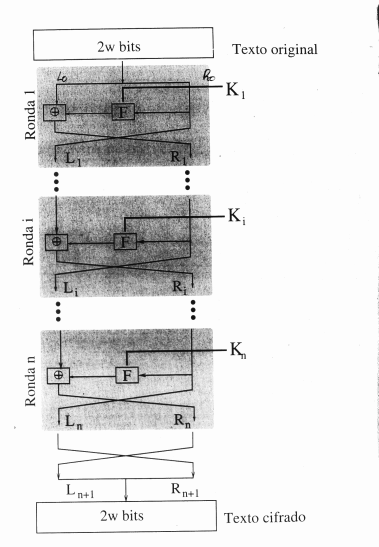
\includegraphics{RondasDES1.png}
 
 \newpage
 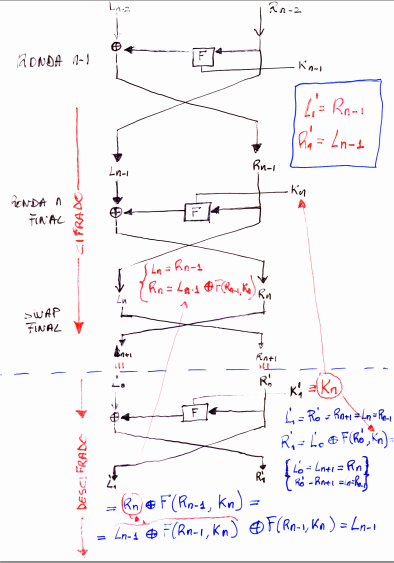
\includegraphics{RondasDES2.png}
 
 \newpage

\subsection{Principios de diseño de las S-Box en DES}

Esta sección también está muy bien explicada en el Stinson, p.79.

\begin{itemize}
	\item Las S no son lineales.
	$$f(x \oplus y) = f(x) \oplus f(y) + cte \implies \text{Esa constante es la que rompe la linealidad}$$
	
	\begin{example}
		\begin{center}
			\begin{tabular}{r  r  r  r  r  r }
				$b_1$ & $b_2$ & $b_3$ & $b_4$ & $b_5$ & $b_6$
			\end{tabular}
		\end{center}
		$$\downarrow$$
		$$\fbox{\textbf{     }S\textbf{     }}$$
		$$\downarrow$$
		\begin{center}
			\begin{tabular}{r  r  r  r }
				$c_1$ & $c_2$ & $c_3$ & $c_4$
			\end{tabular}
		\end{center}
		
		
	\end{example}
	
	\item \textbf{SAC} (Strict avalanch criterion)
	
	Este principio dice que la probabilidad de cambio debe estar equidistribuida.
	
	Esto es, que si cambio un bit de entrada, la probabilidad de que un bit de salida sea 0 o 1 es la misma.
	$$\forall i,j\text{  }P(c_i=1|\overline{b_j})  P(c_i=0|\overline{b_j}) = \frac{1}{2}$$
	Siendo $\overline{b_j}$ que he cambiado el bit $b_j$
	
	\item \textbf{BIC} (bit independence criterion)
	
	Busca que no haya dependencia entre los bits de salida (si cambia $c_3$, no condiciona a que cambie o no $c_2$) 
	$$\forall i,j,k \text{  } P(c_ic_j|\overline{b_k}) = P(c_i|\overline{b_k})\cdot P(c_j|\overline{b_k})$$
	
\end{itemize} 

\subsubsection{Métodos de construcción de las cajas S}
 \begin{itemize}
 	\item \textbf{Aleatorio}
 	\begin{itemize}
 		\item Aleatorio normal
 		\item Con comprobación
 	\end{itemize}
 	\item \textbf{Manual}: El DES utiliza este método
 	\item \textbf{Funciones Matemáticas}: El AES utiliza este método
 \end{itemize}
 
 \subsubsection{Propiedades del DES}
 \begin{itemize}
 	
 
 \item \textbf{Complementaria}: 
 
 Si $y = e_k(x)$ entonces $\overline{y} = e_{\overline{k}}(\overline{x})$.
 
 De esta forma el problema del ataque por texto escogido se reduce a la mitad.
 
 \item \textbf{Claves débiles}(de punto fijo):
 
  Son las claves que cumplen que: $$e_k(e_k(x))= x$$
 
 El DES tiene 4 claves débiles.
 
 \item \textbf{Claves semi-débiles}: 
 
 Son las claves que cumplen que: $$e_{k_1}(e_{k_2}(x)) = x$$
 El DES tiene 6 pares de claves semi-débiles.
 
 \item \textbf{Las claves en DES no forman un grupo}
 
 $$\nexists k_3 \text{ tal que } e_{k_3}(x) = e_{k_1}(e_{k_2}(x))$$
 
\end{itemize}

\subsubsection{Modos de operación del DES}

Hay varias formas de utilizar el DES. Vamos a ver algunas de ellas.

\begin{itemize}
	\item \textbf{ECB}(Electronic Code Book)
	El esquema de funcionamiento del ECB es el siguiente:
	
	\begin{center}
		\Tree[.P [.$P_1$ [.K$\rightarrow\fbox{DES}$ [.$C_1$ [.K$\rightarrow$\fbox{$DES^{-1}$} [.$P_1$ ] ] ] ] ] [.$P_2$ [.K$\rightarrow\fbox{DES}$ [.$C_2$ [.K$\rightarrow$\fbox{$DES^{-1}$} [.$P_2$ ] ] ] ] ]
		[............. ] [.$P_n$ [.K$\rightarrow\fbox{DES}$ [.$C_n$ [.K$\rightarrow$\fbox{$DES^{-1}$} [.$P_n$ ] ] ] ] ] ]
	
	\end{center}
	
	Analizando el ECB nos damos cuenta de que no funciona bien para encriptar mensajes largos ya que los bloques se encriptan de forma independiente.
	
	Esto hace que en lenguajes muy estructurados es muy posible coger bloques iguales que se encriptan igual.
	
	% PONER EL EJEMPLO DE LA IMAGEN ENCRIPTADA CON ECB
	
	\item \textbf{CBC}
	\begin{center}
		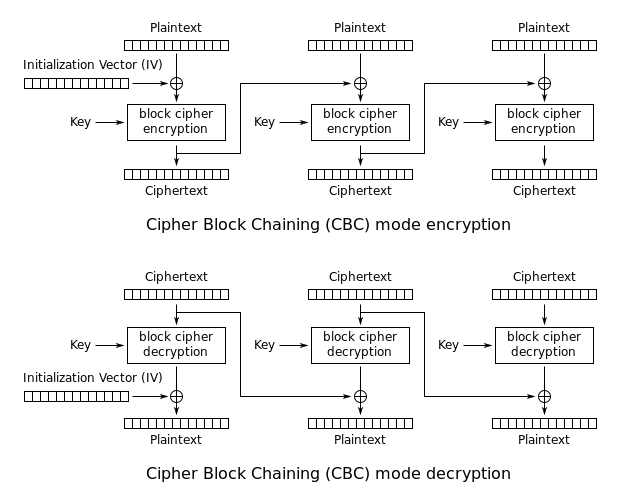
\includegraphics[width=400pt]{CBC.png}
	\end{center}
	 
	
	El IV es el Vector de Inicialización y es secreto.
	
	De esta forma nos queda que:
	$$C_1 = E_K(IV\oplus P_1)$$
	$$C_i = E_K(C_{i-1} \oplus P_i)$$
	$$P_1 = IV \oplus D_K(C_1)$$
	$$P_i = C_{i-1} \oplus D_K(C_i)$$
	
	Analizandolo bit a bit, llamamos $P_1[i]$ al bit i del primer bloque de texto plano.
	
	$$P_1[i] = IV[i] \oplus D_K(C_i)[i]$$
	$$\overline{P_1[i]} = \overline{IV[i]} \oplus D_K(C_i)[i]$$
	
	Este cifrado no tiene el mismo problema que el ECB ya que encripto $P_i$ en función de lo que me devuelva al encriptar $P_{i-1}$ , es decir, que voy cambiando la semilla.
	
	\item \textbf{CFB}
	\item \textbf{OFB}
	\item \textbf{CTR}
	\begin{center}
		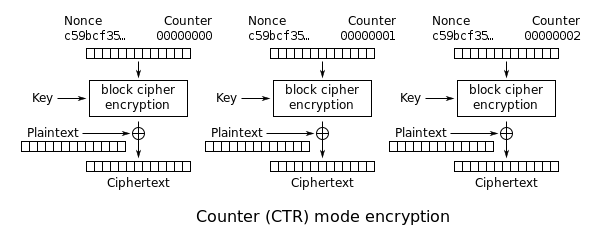
\includegraphics[width=400pt]{CTR.png}
	\end{center}
	\textbf{Características del CTR}
	\begin{itemize}
		\item No cifra igual trozos iguales
		\item No utiliza $DES^{-1} \rightarrow$ genial para implementar
		\item No hace falta hacer las operaciones en cadena ya que ahora dependemos de una clave que va cambiando $\rightarrow $ el contador
	\end{itemize}
		\textbf{Ventajas del CTR}
		\begin{itemize}
			\item Preproceso $\rightarrow$ puedo calcular todos los contadores + DES antes de leer el texto. 
			\item Acceso aleatorio
			\item Simplicidad
		\end{itemize}
	
\end{itemize}

\chapter{DES DOBLE}
Debido a lo vulnerable que es el DES se buscaron posibles alternativas. Una de ellas es la encriptación múltiple, en la cual el algoritmo de encriptación se usa varias veces sobre el mismo texto recibiendo como entrada la enciptación aterior.

\section{Funcionamiento DES doble}
Tenemos un texto plano P y dos claves $K_1$, $K_2$
$$C= DES_{K_2}(DES_{K_1}(P))$$
$$P = DES^{-1}_{K_1}(DES^{-1}_{K_2}(C)) \implies DES_{K_1}(P) = DES^{-1}_{K_2}(C)$$

Además tiene la propiedad de que:
$$DES_{K_3}(x) \neq DES_{K_2}(DES_{K_1}(x))$$

Según esto, como $K_1$ y $K_2$ son de 64 bits , aparentemente la robusted de la clave es $64 \cdot 2 = 128$

\section{Robusted DES DOBLE}

Vamos a ver cómo descubrir las claves utilizadas en el caso de tener un par (P,C) conocido.

Utilizando la igualdad $DES_{K_1}(P) = DES^{-1}_{K_2}(C)$:
\begin{enumerate}
	\item Escribimos en una tabla la encriptación de P con los $2^{56}$ posibles valores de $K_1$ (hemos quitado los bits de paridad, por eso no es $2^64$).
	
	\item Escribimos en otra tabla la desencriptación de C con los $2^{56}$ posibles valores de $K_2$
	
	\item Vemos las claves con las que hay coincidencia
	
\end{enumerate} 

El coste de este proceso ha sido ejecutar $2 \cdot 2^{56} = 2^{57}$ veces el DES, más el tiempo en hacer las comparaciones (que es despreciable).

Por lo tanto la robusted del DES doble es aproximadamente $2^{57}$

Pero esto es muy poco, vamos a ver el DES Triple

 % % Me faltan infinitas hojas % %
 
 \chapter{Triple DES}
 El triple DES es otra alternativa de encriptación múltiple.
 
 Hay dos tipos de Triple DES:
 \begin{enumerate}
 	\item Triple DES de \textbf{2 claves}
 	\item Triple DES de \textbf{3 claves}
 \end{enumerate}
 \section{Funcionamiento Triple DES de 2 claves}
 Tenemos un texto plano P y dos claves $K_1$ , $K_2$, de 64 bits cada una, es decir 128 bits, que si quitamos los bits de paridad se quedan en 112 bits.
 
 $$C = DES_{K_1}(DES^{-1}_{K_2}(DES_{K_1}(P)))$$
 
 $$P = DES^{-1}_{K_1}(DES_{K_2}(DES^{-1}_{K_1}(P)))$$
 
 Esto hace que no sea posible el ataque que habíamos visto en el DES Doble ya que
 $$DES_{K_1}(P) = DES_{K_2}(DES^{-1}_{K_1}(C))$$
 
 \section{Funcionamiento Triple DES de 3 claves}
 
 En este caso el algoritmo de encriptación es:
 $$C = DES_{K_3}(DES^{-1}_{K_2}(DES_{K_1}(P )))$$
 
 \begin{example}
 	Queremos demostrar que 
 	$$DES_K(x) = \overline{DES_{\overline{K}}(\overline{x})}$$
 	
 	Para esto complementamos los dos lados e la igualdad de forma que nos queda
 	$$\overline{DES_K(x)} = DES_{\overline{K}}(\overline{x})$$
 	
 	Ahora vamos a desarrollar la parte derecha:
 	$$DES_{\overline{K}}(\overline{x}) \implies \begin{cases}
		L_1 = \overline{R_0}\\
		R_1 = \overline{L_0} \oplus F(\overline{R_0} , \overline{K_1})
 	\end{cases}$$
 	
 	Sabemos que $F(\overline{R_0} , \overline{K_1}) = E(\overline{R_0}) \oplus \overline{K_1}$
 	
 	Al ser E $\rightarrow$ expansión, vemos que 
 	$$E(\overline{R_0}) = \overline{E(R_0)}$$
 	
 	Y además una propiedad del XOR es que
 	$$a\oplus b = \overline{a} \oplus \overline{b}$$
 	
 	por tanto
 	$$E(\overline{R_0}) \oplus \overline{K_1} = \overline{E(R_0)} \oplus \overline{K_1} = E(R_0) \oplus K_1$$
 	
 	Según lo que acabamos de calcular
 	$$DES_{\overline{K}}(\overline{x})\begin{cases}
	 	R_1 = \overline{L_0} \oplus F(\overline{R_0} , \overline{K_1}) = \overline{L_0} \oplus F(R_0 , K_1)\\
	 	\overline{R_0} = L_1
 	\end{cases}$$
 	
 	Si ahora complementamos esto:
 	$$\overline{DES_{\overline{K}}(\overline{x})}\begin{cases}
 	\overline{R_1} = L_0 \oplus F(\overline{R_0} , \overline{K_1}) = L_0 \oplus F(R_0 , K_1) = R_1\\
 	\overline{L_1} = R_0 = L_1
 	\end{cases}$$
 	
	Y asi vemos que se cumple la igualdad 	
 \end{example}
 \newpage
 
 
 
 $$D(x) = C(x) \text{ mod M(x)} \begin{cases}
 d_0 = a_0\cdot b_0 \oplus a_3 \cdot b_1 \oplus a_2 \cdot b_2 \oplus a_1 \cdot b_3 = C_0 \oplus C_4\\
 d_1 = a_1\cdot b_0 \oplus a_0 \cdot b_1 \oplus a_3 \cdot b_2 \oplus a_2 \cdot b_3 = C_1 \oplus C_5\\
 d_2 = a_2\cdot b_0 \oplus a_1 \cdot b_1 \oplus a_0 \cdot b_2 \oplus a_3 \cdot b_3 = C_2 \oplus C_6\\
 d_3 = a_3\cdot b_0 \oplus a_2 \cdot b_1 \oplus a_1 \cdot b_2 \oplus a_0 \cdot b_3 = C_3
 \end{cases}$$
 
 $$\left(\begin{matrix}
 d_0\\d_1\\d_2\\d_3
 \end{matrix} \right) = \left(\begin{matrix}
 a_0 & a_3 & a_2 & a_1\\
 a_1 & a_0 & a_3 & a_2\\
 a_2 & a_1 & a_0 & a_3\\
 a_3 & a_2 & a_1 & a_0\\
 \end{matrix}\right) \cdot \left( \begin{matrix}
 b_0\\
 b_1\\
 b_2\\
 b_3
 \end{matrix}\right)$$
 
 Esta operación esta definida  anivel de W (palabra).
 
 \section{Multiplicación por X}
 
 $$XTIME = x \cdot b(x) = b_3x^4 + b_2 x^3 + b_1 x^2 + b_0 x \textbf{ mod M(x)} = b_2x^3 +b_1x^2 + b_0x + b_3$$
 
 Vemos que esto lo que hace es un desplazamiento cíclico (rotación).
 
 $$XTIME(b_3 b_2 b_1 b_0) = b_2 b_1 b_0 b_3$$
 
 
 $$C(x) = x \cdot b(x) = \left(\begin{matrix}
 	C_0\\C_1\\C_2\\C_3
 \end{matrix} \right) = \left(\begin{matrix}
 00 & 00 & 00 & 01\\
 01 & 00 & 00 & 00\\
 00 & 01 & 00 & 00\\
 00 & 00 & 01 & 00\\
\end{matrix}\right) \cdot \left( \begin{matrix}
b_0\\
b_1\\
b_2\\
b_3
\end{matrix}\right)$$
 
 
\section{Diseños y criterios para el AES}

\subsubsection{Objetivos}

\begin{itemize}
	\item Resistente al C.D y C.L (criptoanálisis diferencial y lineal)
	\item Eficiente en varias plataformas
	
	Cumple este objetivo porque las operaciones son sumas, rotaciones y desplazamientos, que son operaciones que soporta cualquier plataforma informática. Y al ser de tan bajo nivel son my rápidas
	
	\item Código compacto y sencillo
	\item Fuerte base matemática
\end{itemize}

\subsubsection{Elementos de Diseño}

\begin{itemize}
	\item Capa lineal $\rightarrow$ Difusión
	\item Capa no lineal $\rightarrow$ Confusión
	
	Esto es antes de mezclarse la clave
	\item Capa de sumas de clave
	\item Clave variable $\rightarrow$ 128, 192, 256
	\item Bloque variable $\rightarrow$ 128, 192, 256
	
	El tamaño de bloque estándar es 128.
\end{itemize}

A pesar de utilizar los principios de confusión y difusión no es una esructura Feistel clásica.
 
\subsubsection{Diseño de Rijndael}

STATE (estado)

$$\overrightarrow{X} = x_0 , ...., x_n$$

$$x_i \in GF(2^8)|m(x)$$

Antes de estrar en el algoritmo se coloca este string en bloques para que el algoritmo pueda operar con él.

Se coloca de la siguiente forma:

Se pasa de esta notación:

	\begin{center}
		\begin{tabular}{l | l | c | r | r | r}
			$x_0$ & $x_4$ &  &  &  &  \\
			\hline
			$x_1$  & $x_5$ &  &  &  &  \\
			\hline
			$x_2$  &  &  &  &  &  \\
			\hline
			$x_3$ &  &  &  &  & $x_{23}$ \\
		\end{tabular}
	\end{center}
	
	$$\begin{cases}
	N_B = 4 \rightarrow 128\\
	N_B = 6 \rightarrow 192\\
	N_B = 8 \rightarrow 256\\
	\end{cases}$$

A esta notación	


	\begin{center}
		
		\begin{tabular}{l | c | r | r | r | r}
			$a_{00}$ & $a_{01}$ & $a_{02}$ & $a_{03}$ & $a_{04}$ & $a_{05}$\\
			\hline
			$a_{10}$ &   &   &   &   &  \\
			\hline
			$a_{20}$ &   &   &   &   &  \\
			\hline
			$a_{30}$ &   &   &   &   & $a_{35}$
			
		\end{tabular}
	\end{center}


\subsubsection{Tamaño de clave}

	\begin{center}
		
		\begin{tabular}{l | c | r | r }
		$K_{00}$ & $K_{01}$ & $K_{02}$ & $K_{03}$\\
		\hline
		$K_{10}$ &  &  & \\
		\hline
		$K_{20}$ &  &  & \\
		\hline
		$K_{30}$ &  &  & $K_{33}$
		
		\end{tabular}
	\end{center}
	
		$$\begin{cases}
		N_K = 4 \rightarrow 128\\
		N_K = 6 \rightarrow 192\\
		N_K = 8 \rightarrow 256\\
		\end{cases}$$
		
\subsubsection{Número de rondas}
	\begin{center}
		
		\begin{tabular}{l | c | r | r }
		$N_K$ & $N_B$ = 4 & $N_B$ = 6 & $N_B$ = 8\\
		\hline
		$N_K$ =4 &  10 & 12 & 14\\
		\hline
		$N_K$ = 6 & 12 & 12 & 14\\
		\hline
		$N_K$=8 & 14 & 14 & 14
		
		\end{tabular}
	\end{center}

\subsubsection{Una ronda AES}
\lstset{language=C, breaklines=true, basicstyle=\footnotesize}
\begin{lstlisting}[frame=single]

	Round(state , Subkey){
	
		ByteSub (STATE) ; //equivalente a S_Box, operaciones $GF(2^8)$, bit a bit
	
		ShiftRow(STATE); // desplazamiento de filas del STATE (operaciones W)
	
		MIXCOLUMN (STATE); // Operaciones con columnas utilizando W
	
		AddRoundKey (STATE, SubKey);
	} 
	
	+
	 
	FinalRound(S,SK){
		ByteSub(S);
		ShiftRow(S);
		AddRoundKey(S,SK);
	}
		
\end{lstlisting}

Ahora vamos a analizar cada una de las \textbf{funciones del AES}
\begin{itemize}
	\item \textbf{ByteSub}:
	Supongamos que el STATE ya lo tenemos como:
	
	\begin{center}
		
		\begin{tabular}{l | c | r | r | r | r}
			$a_{00}$ & $a_{01}$ & $a_{02}$ & $a_{03}$ & $a_{04}$ & $a_{05}$\\
			\hline
			$a_{10}$ &   &   &   &   &  \\
			\hline
			$a_{20}$ &   &   &   &   &  \\
			\hline
			$a_{30}$ &   &   &   &   & $a_{35}$
			
		\end{tabular}
	\end{center}
	
	en la función tenemos 3 pasos
	\begin{enumerate}
		\item Calculamos el \textbf{inverso multiplicativo de cada cada byte} $a_{ij}$
		
		$$a_{ij} \rightarrow a'_{ij}$$
		
		Para esto tenemos un convenio que es que el inverso de $00$ es $00$, ya que en realidad el 0 no tiene inverso multiplicativo.
		
		\item Se calcula la \textbf{transformación afín} $y = ax +b$ de cada $a'_{ij}$
		
		Esta transformación es una especie de difusión, tipo Hill.
	\end{enumerate}
	
	¿Cuantos ByteSub posibles podemos calcular? Vemos que es una función de byte, es decir, el parámetro es un byte , por lo tanto tenemos 256($2^8$) posibilidades.
	
	Los resultados de cada byte se guardan en las tablas de sustitución, las cajas-S del AES.
	$$S-BOX[a_{ij}] = b_{ij}$$
	
	Esta cajas S cogen los 4 primeros bits, que le indican la columna, y los 4 últimos bits le indican la fila.
	
	¿Cómo funciona la función inversa? \textbf{INVByteSub}:
	\begin{enumerate}
		\item Se calcula la\textbf{transformación afín INVERSA}, que viene determinada por (imagen de moodle matriz Y)
		\item Se calcula el \textbf{inverso multiplicativo del resultado}
	\end{enumerate}
	
	De la función inversa también surge una caja de sustitución. La \textbf{Inverse S-Box}
	$$S-BOX^{-1}[b_{ij}] = a_{ij}$$
	\textbf{DISEÑO DE LAS S-BOX DEL AES}
	\begin{itemize}
		\item Resistentes al $\begin{cases}
			\text{C.D Criptoanálisis diferencial}\\
			\text{C.L Criptoanálisis lineal}
		\end{cases}$
		
		Es decir, que casi no hay correlación entre los bits de entrada y los de salida.
		
		\item No existen los puntos fijos. Para esto juegan un papel muy importante las constantes c y d que vemos en las matrices de ejemplo que hemos puesto anteriormente.
		
		\item Las S-BOX tienen inversa: 
		$$IS-BOX[S-BOX(a)] = a$$
		Además $$S-BOX[a]\neq IS-BOX[a]$$
		
		Por ejemplo:
		 $$S-BOX(95) = 2A$$
		 $$IS-BOX[95]=  AD$$
	\end{itemize}
	Ejercicio para casa: intentar calcular el ByteSub de '95'. Solución= '2A'
\end{itemize}
